\section{Introduction}

[TO DO]

\paragraph{Dark matter general}
\begin{itemize}
\item The flat rotation curves of galaxies were the first indication, that galaxies could reside in large and massive, more or less spherical halos made of invisible dark matter $\longrightarrow$ stellar movements in solar neighbourhood \citep{1932BAN.....6..249O}, $H\alpha$ rotation curves of external galaxies \citep{1978ApJ...225L.107R}
\item Standard model of cosmology, based on the by the Planck Mission, predicts $\sim32\%$ of the universes content is in the form of matter and $\sim 85\%$ of the total matter is non-baryonic dark matter.
\end{itemize}

\paragraph{Lensing to measure mass}
\begin{itemize}
\item Completely independent method to measure mass of galaxies is gravitational lensing
\item massive galaxies can act as gravitational lenses, deflect light of background sources, gives rise to multiple images
\item By 2010 over 200 strong gravitational galaxy lenses had been discovered \citep{2010ARA&A..48...87T} and the number is still rising
\item On galaxy scales strong gravitational lensing is sensitive to the total projected matter amount inside approximately $\sim 1$ arcsec.
\end{itemize}

\paragraph{Dynamical modelling to measure mass}
\begin{itemize}
\item Gas rotation curves are useful to measure matter distribution at large radii
\item gas on circular orbits $\longrightarrow$ directly circular velocity curve and mass profile. 
\item But: gas has dissipative nature, concentrated to mid-plane $\longrightarrow$ sensitive to disturbances by e.g. bars, spiral arms
\item stars are dissipationless, present almost everywhere in the galaxy $\longrightarrow$ very good tracers of the underlying gravitational potential $\longrightarrow$  but much more complex motions: bulk rotation around principal axis, plus random motion components in all coordinate directions $\longrightarrow$ velocity anisotropy $\longrightarrow$ degeneracy with matter distribution 
\item modelling: account for stellar rotation, dispersion and velocity anisotropy
\item e.g. solution of the Jeans equations for an assumed velocity anisotropy, e.g. \citet{Cap08}
\item dynamical modelling of stellar kinematics also at smaller radii $\longrightarrow$ complement lensing investigation of the matter distribution in the center of galaxies
\item Other modelling methods: Schwarzschild's orbital superposition approach \citep{schwarzschild}
\end{itemize}

\paragraph{Dark Matter Halos}
\begin{itemize}
\item Cosmological cold dark matter N-body simulations suggest that dark matter halos take a cuspy shape, following a NFW profile \citep{NFW96}
\item central dark matter density cusps are not observed in dark matter dominated galaxies (dwarfs); if they exist in more massive galaxies depends strongly on stellar mass-to-light ratio. Overall, observations suggest cored dark matter halos $\longrightarrow$ core-cusp problem, might be due to a yet unknown interaction between dark matter and baryons
\end{itemize}

\paragraph{SWELLS Survey}
\begin{itemize}
\item [TO DO]
\item Sloan WFC Edge-on Late-type Lens Survey (SWELLS) WFC = Wide field camera \citep{SWELLSI,SWELLSII,SWELLSIII,SWELLSIV,SWELLSV,SWELLSVI}
\item \citet{SWELLSI} give measurements for the apparent AB magnitudes for the HST/WFPC2 I-band/F814W filter for disk and bulge, as well as stellar masses for stellar population models for a Chabrier [TO DO: REF] and Salpeter [TO DO: REF] initial mass function (IMF). 
\item dedicated to find spiral galaxy strong lenses, to combine lensing and dznamical modelling to break degeneracies inherent in both methods.
\item picked galaxies in SDSS whose spectra had to different redshifts within 3 arcsec, which makes it likely to capture strong lenses with typical Einstein radii of 1 arcsec. Sufficiently inclined galaxies were picked by eye. Follow up high resolution imaging with the Hubble Space Telescope's (HST) Wide-Field Planetary Camera 2 (WFPC2) was performed \citep{SWELLSI}).
\end{itemize}


\paragraph{Characteristics of J1331}
\begin{itemize}
\item SDSS J1331+3638 (J1331)
\item approximate hubble type Sb, Spiral galaxy almost edge-on
\item first discovered by Sloan digital sky survey (SDSS) [TO DO: REF]
\item \citet{SWELLSI} identified it as a strong lens
\item Its coordinates on the sky are right ascension = 202.91800$^\circ$ and a declination = 36.46999$^\circ$ (epoch J2000). 
\item This galaxy is at a redshift of $z_d = 0.113$ (\cite{SWELLSIII}).
\item large reddish bulge and bluish spiral arms, see Fig. \ref{fig:F450W} and \ref{fig:F814W}
\item superimposed by quadruplet of extended bluish images at a redshift of $z_s\simeq0.254$ [TO DO: REF], see Fig. \ref{fig:lens_just_imgpos}, approximately at a distance of 1 arcsec from the galaxy center (which is a typical Einstein radius).
\item Lens image redshift $z_s = 0.254$  \citep{SWELLSIII}
\item lensed object might be a star-forming blob of a background galaxy.
\item Lensing properties first analysed by \citet{SWELLSIII}
\item rather edge-on $\longrightarrow$ possible to measure rotation curves. \citet{SWELLSV} measured the gas and stellar rotation curves along the major axis. Fitted galaxy model to gas kinematics at large radii, and lensing result
\item large counter-rotating core, see Fig. \ref{fig:kinematics}
\item possible minor merger in the past
\item background object: possibly bright star forming region in the spiral arms of background galaxy 
\end{itemize}

\paragraph{Goal of this work}
\begin{itemize}
\item constraining the matter distribution in a galaxy, disentangling stellar and dark matter component at smaller radii
\item using two independent methods, lensing and dynamics
\item testing, if Jeans modelling works also in the presence of counter-rotating cores
\item focus on the smaller radii, as \citet{SWELLSV} was focusing on outer regions
\item complementing the work by [SWELLS paper on lensing and lensing/dynamcis TO DO: find] by an in depth analysis
\item ideal case: investigating how a minor merger modifies the mass distribution of a galaxy
\end{itemize}


\paragraph{Data used}
\begin{itemize}
\item Hubble Space Telescope (HST)/WFPC2/WFC3 imaging by \cite{SWELLSI}, see Fig. \ref{fig:F450W} and \ref{fig:F814W}
\item  \citet{SWELLSV} measured the gas and stellar rotation curves along the major axis. see Fig. \ref{fig:F814W} and \ref{fig:kinematics}
\end{itemize}

\paragraph{Methods}
\begin{itemize}
\item similar analysis of J1331 as \citet{GlennEC} has done with the Einstein cross
\item lensing: fitting scale-free galaxy model to image positions \citep{EvansWitt}
\item photometry: MGE expansion of surface brightness in the F814W filter (deconvolution with PSF), apparent magnitude, total luminosity, effective radius
\item Jeans modelling: jeans axisymmetric modelling (JAM) by \citet{Cap08} to fit model predictions for the second velocity moments to the stellar kinematics data
\end{itemize}

[TO DO]


%============================================================================


\begin{figure*}
\centering
\begin{subfigure}{.5\textwidth}
  \centering
  \includegraphics[width=.9\linewidth]{fig/first_glimpse_450.ps}
  \caption{J1331 in F450W ("blue")}
  \label{fig:F450W}
\end{subfigure}%
\begin{subfigure}{.5\textwidth}
  \centering
  \includegraphics[width=.9\linewidth]{fig/first_glimpse_814.ps}
  \caption{J1331 in F814W ("red")}
  \label{fig:F814W}
\end{subfigure}
\begin{subfigure}{.5\textwidth}
  \centering
  \includegraphics[width=.9\linewidth]{fig/lens_imgpos.ps}
  \caption{The lensing images}
  \label{fig:lens_just_imgpos}
\end{subfigure}%
\begin{subfigure}{.5\textwidth}
  \centering
  \includegraphics[width=.9\linewidth]{fig/stellar_kinematics_data.ps}
  \caption{Stellar Kinematics by \citet{SWELLSV}}
  \label{fig:kinematics}
\end{subfigure}
\caption{Hubble Space telescope (HST) images and stellar kinematics of the galaxy SDSS J1331+3638 (J1331), which has a large counter-rotating core and whose bulge acts as a strong lens for a bluish background source. \emph{Panel (a) and (b):} HST/WFPC2/WFC3 images of J1331 by \citet{SWELLSI} in two filters, F450W in panel (a) and F814W in panel (b). The galaxy's coordinates on the sky are right ascension $\alpha$ = 202.91800$^\circ$ and declination $\delta$ = 36.46999$^\circ$ (epoch J2000). Image orientation and scaling are indicated in panel (a); the scaling transformation from arcseconds to the physical size of the galaxy in kpc uses the galaxy's redshift $z_d = 0.113$ \citep{SWELLSIII} (i.e. assumes an angular diameter distance of 414 Mpc). The color scaling of these two images is the same. The black solid line in panel (b) shows the orientation of the major-axis. The line has a length of 10 arcsec and indicates the region within which we carry out the Jeans modelling. [TO DO: NOT ALL THE TIME.???????] \emph{Panel (c):} The central region of J1331 in F450W, surface brightness subtracted. An IRAF ellipse ???? fit to the F450W surface brightness in panel (a) was subtracted from the image. The (smoothed) residuals within the white square in panel (a) are shown in panel (c). Four bright blobs (A,B,C and D) become visible, which are arranged in a typical strong lensing configuration around the center of the galaxy (G). \emph{Panel (d):} Stellar Kinematics along the galaxy's major axis as measured by \citet{SWELLSV}, line-of-sight rotation velocity $v_\text{rot}$, line-of-sight velocity dispersion $\sigma$ and the rms-velocity $v_\text{rms} = \sqrt{v_\text{rot}^2 + \sigma^2}$. The dotted line in panel (b) indicates the galaxy's effective half-light radius (in the F814W filter), $R_\text{eff} = 2.6" = 5.2$ kpc. The $v_\text{rot}$ curve reveals that J1331 is counter-rotating within $R_\text{eff}$. [TO DO: Add (x,y) axis in figure b).???????]}
\label{fig:specialJ1331}
\end{figure*}